\subsection{Ablations}

\subsubsection{Renorm / CLIP comparisons}

Tables \ref{tab:renorm_clip_table_dogstocats} show results with and without the renormalization step and with or without the clipping step.

The renormalization step is introduced in the same way as for CASteer:

\begin{align*}
    \hat{h}_{norm} = \frac{f(h)}{\norm{f(h)}} \cdot \norm{h}    
\end{align*}
, where $f$ is a steering function (either CASteer, LEACE or MidSteer).


For clipping, first let us notice that when considering either LEACE, CASteer or MidSteer, any transformation $f(h) = Ah + b$ has the form:

\begin{align*}
    A &= I - \beta U V^T \\
    b &= c - Ac \\
    f(h) &= A (h-c) + c = h - \underbrace{\beta UV^T \tilde{h}}_{=\Delta}
\end{align*}

, for some $c \in \mathbb{R}^d$, and $U, V \in \mathbb{R}^{d \times k}$ and $\tilde{h} = h - c$. Here, for CASteer $c=0$ and $U = V = s$. For LEACE and MidSteer, $c=\mathbb{R}[X]$ and $U, V$ are defined in theorems.

We introduce clipping in a similar way as for CASteer: $f(h) = h - \beta U \max(V^T \tilde{h}, 0)$. The reason behind this is that $V^T u$ in all methods computes such vector $a$ s.t. $Cov(a^T, X)$ is as close to $u$ as possible. In other words, it computes per concept linear regression coefficients for $Z$. And we want to nullify those concepts which are not present, or present in negative form.

The results for this can be found in \ref{tab:renorm_clip_table_dogstocats} and \ref{tab:renorm_clip_table_horsestomotorcycles}. As can be seen, renormalization does not help either method much, so the next tables will be presented without it.


Clipping helps CASteer and LEACE more because in the LLM setup for $\beta=2$ they can oscillate back and forth for alternating tokens. Clipping also improves the results of MidSteer on Alpaca and MMLU, signifying that it helps mitigate unwanted changes in real-life scenarios where concrete concepts are not present. Since MidSteer already exhibits good results on these datasets, and without clipping it can be re-written in pure matrix-multiplication form (without altering the architecture of a neural network), we will present results on MidSteer without clipping.



\begin{table}[htbp]
\centering
\caption{Renorm/Clip Comparison - Dogs$\to$Cats}
\label{tab:renorm_clip_table_dogstocats}
\begin{tabular}{l|c|c|c|cccccc|}
\hline
Method & $\beta$ & Renorm & Clip & \multicolumn{6}{c|}{Metrics} \\
 &  &  &  & SCS & TCS & A-BLEU & A-BertF1 & M-BLEU & M-BertF1 \\
\hline
Baseline & — & \checkmark & \checkmark & \textbf{8.67} & 1.02 & — & — & — & — \\
 &  &  & \checkmark & \underline{8.67} & 0.99 & — & — & — & — \\
 &  & \checkmark &  & 8.66 & 1.03 & — & — & — & — \\
 &  &  &  & 8.60 & 0.96 & — & — & — & — \\
\hline
CASteer & 2.0 & \checkmark & \checkmark & 4.57 & 5.77 & 0.776 & 0.976 & 0.756 & 0.968 \\
 &  &  & \checkmark & 4.73 & 5.64 & 0.777 & 0.976 & 0.752 & 0.968 \\
 &  & \checkmark &  & 5.90 & 4.03 & 0.670 & 0.965 & 0.557 & 0.942 \\
 &  &  &  & 5.95 & 3.93 & 0.669 & 0.964 & 0.558 & 0.942 \\
\hline
LEACE & 2.0 & \checkmark & \checkmark & 3.55 & 6.37 & 0.886 & 0.989 & \underline{0.881} & \underline{0.984} \\
 &  &  & \checkmark & 3.42 & 6.40 & 0.886 & 0.988 & \textbf{0.882} & \textbf{0.985} \\
 &  & \checkmark &  & 4.10 & 5.50 & 0.863 & 0.986 & 0.790 & 0.972 \\
 &  &  &  & 3.94 & 5.53 & 0.862 & 0.986 & 0.786 & 0.972 \\
\hline
Mean Matching & 2.0 & \checkmark & \checkmark & 2.56 & 7.60 & \underline{0.900} & \underline{0.990} & 0.791 & 0.973 \\
 &  &  & \checkmark & 2.46 & \textbf{7.72} & 0.899 & \textbf{0.990} & 0.789 & 0.972 \\
 &  & \checkmark &  & 2.57 & 7.63 & \textbf{0.900} & 0.990 & 0.791 & 0.973 \\
 &  &  &  & 2.59 & \underline{7.71} & 0.899 & 0.990 & 0.786 & 0.972 \\
\hline
\end{tabular}
\end{table}

\begin{table}[htbp]
\centering
\caption{Renorm/Clip Comparison - Horses$\to$Motorcycles}
\label{tab:renorm_clip_table_horsestomotorcycles}
\begin{tabular}{l|c|c|c|cccccc|}
\hline
Method & $\beta$ & Renorm & Clip & \multicolumn{6}{c|}{Metrics} \\
 &  &  &  & SCS & TCS & A-BLEU & A-BertF1 & M-BLEU & M-BertF1 \\
\hline
Baseline & — & \checkmark & \checkmark & 8.65 & 0.60 & — & — & — & — \\
 &  &  & \checkmark & \textbf{8.67} & 0.57 & — & — & — & — \\
 &  & \checkmark &  & 8.66 & 0.55 & — & — & — & — \\
 &  &  &  & \underline{8.67} & 0.60 & — & — & — & — \\
\hline
CASteer & 2.0 & \checkmark & \checkmark & 2.11 & \underline{7.64} & 0.754 & 0.974 & 0.646 & 0.954 \\
 &  &  & \checkmark & 2.16 & \textbf{7.67} & 0.753 & 0.974 & 0.647 & 0.954 \\
 &  & \checkmark &  & 2.74 & 6.91 & 0.668 & 0.964 & 0.555 & 0.942 \\
 &  &  &  & 2.65 & 6.93 & 0.664 & 0.964 & 0.560 & 0.943 \\
\hline
LEACE & 2.0 & \checkmark & \checkmark & 4.48 & 4.98 & \underline{0.873} & \underline{0.987} & \underline{0.803} & \underline{0.974} \\
 &  &  & \checkmark & 4.71 & 4.63 & \textbf{0.875} & \textbf{0.987} & \textbf{0.806} & \textbf{0.975} \\
 &  & \checkmark &  & 5.24 & 3.70 & 0.852 & 0.985 & 0.777 & 0.971 \\
 &  &  &  & 5.37 & 3.64 & 0.851 & 0.985 & 0.780 & 0.971 \\
\hline
Mean Matching & 2.0 & \checkmark & \checkmark & 2.62 & 7.17 & 0.870 & 0.987 & 0.703 & 0.961 \\
 &  &  & \checkmark & 2.57 & 7.22 & 0.865 & 0.986 & 0.701 & 0.961 \\
 &  & \checkmark &  & 2.54 & 7.17 & 0.872 & 0.987 & 0.698 & 0.960 \\
 &  &  &  & 2.62 & 7.22 & 0.872 & 0.987 & 0.701 & 0.961 \\
\hline
\end{tabular}
\end{table}

\subsubsection{Raw results}

The raw results for different experiments and strengths of the method are presented in the following tables:
\begin{itemize}
    \item No renormalization, with clipping, steering dogs to cats: \ref{tab:single_experiment_table_with_clipping_dogs_to_cats}

    \item No renormalization, with clipping, steering horses to motorcycles: \ref{tab:single_experiment_table_with_clipping_horses_to_motorcycles}

    \item No renormalization, without clipping, steering dogs to cats: \ref{tab:single_experiment_table_without_clipping_dogs_to_cats}

    \item No renormalization, without clipping, steering horses to motorcycles: \ref{tab:single_experiment_table_without_clipping_horses_to_motorcycles}
\end{itemize}


\begin{table}[htbp]
\centering
\caption{Comprehensive Results: midsteer\_sa\_fix\_50k\_last\_no\_renorm\_clip\_all\_strengths - Dogs$\to$Cats}
\label{tab:single_experiment_table_with_clipping_dogs_to_cats}
\begin{tabular}{l|l|cccccc|}
\hline
Method & $\beta$ & \multicolumn{6}{c|}{Dogs$\rightarrow$Cats} \\
 &  & SCS & TCS & A-BLEU & A-BertF1 & M-BLEU & M-BertF1 \\
\hline
Baseline & — & \textbf{8.67} & 0.99 & — & — & — & — \\
\hline
CASteer & 1.0 & \underline{8.58} & 1.10 & 0.856 & 0.985 & 0.855 & 0.981 \\
 & 1.5 & 7.84 & 2.44 & 0.813 & 0.980 & 0.801 & 0.974 \\
 & 2.0 & 4.73 & 5.64 & 0.777 & 0.976 & 0.752 & 0.968 \\
 & 2.5 & 3.70 & 6.55 & 0.744 & 0.972 & 0.717 & 0.963 \\
 & 3.0 & 3.16 & 7.08 & 0.711 & 0.969 & 0.684 & 0.959 \\
 & 3.5 & 2.90 & 7.23 & 0.685 & 0.966 & 0.648 & 0.954 \\
 & 4.0 & 2.73 & 7.42 & 0.658 & 0.963 & 0.616 & 0.950 \\
 & 4.5 & 2.70 & 7.70 & 0.636 & 0.960 & 0.593 & 0.947 \\
 & 5.0 & 2.48 & 7.85 & 0.615 & 0.958 & 0.572 & 0.944 \\
\hline
LEACE & 1.0 & 8.49 & 1.30 & \underline{0.928} & \underline{0.993} & \textbf{0.931} & \textbf{0.991} \\
 & 1.5 & 5.20 & 4.78 & 0.911 & 0.991 & \underline{0.904} & \underline{0.988} \\
 & 2.0 & 3.42 & 6.40 & 0.886 & 0.988 & 0.882 & 0.985 \\
 & 2.5 & 3.04 & 7.25 & 0.871 & 0.987 & 0.860 & 0.982 \\
 & 3.0 & 2.64 & 7.42 & 0.852 & 0.985 & 0.837 & 0.979 \\
 & 3.5 & 2.57 & 7.54 & 0.833 & 0.983 & 0.819 & 0.976 \\
 & 4.0 & 2.47 & 7.76 & 0.822 & 0.982 & 0.802 & 0.974 \\
 & 4.5 & 2.40 & 7.72 & 0.811 & 0.980 & 0.783 & 0.972 \\
 & 5.0 & 2.24 & 7.87 & 0.797 & 0.979 & 0.772 & 0.970 \\
\hline
Mean Matching & 1.0 & 8.04 & 1.85 & \textbf{0.938} & \textbf{0.994} & 0.885 & 0.985 \\
 & 1.5 & 4.24 & 5.91 & 0.916 & 0.992 & 0.833 & 0.978 \\
 & 2.0 & 2.46 & 7.72 & 0.899 & 0.990 & 0.789 & 0.972 \\
 & 2.5 & 2.10 & 8.18 & 0.883 & 0.988 & 0.756 & 0.968 \\
 & 3.0 & 1.90 & 8.42 & 0.874 & 0.987 & 0.727 & 0.964 \\
 & 3.5 & 1.77 & 8.49 & 0.856 & 0.985 & 0.697 & 0.960 \\
 & 4.0 & 1.60 & \textbf{8.59} & 0.837 & 0.983 & 0.669 & 0.957 \\
 & 4.5 & 1.65 & 8.55 & 0.824 & 0.982 & 0.642 & 0.953 \\
 & 5.0 & 1.66 & \underline{8.57} & 0.810 & 0.980 & 0.616 & 0.950 \\
\hline
\end{tabular}
\end{table}

\begin{table}[htbp]
\centering
\caption{Comprehensive Results: midsteer\_sa\_fix\_50k\_last\_no\_renorm\_clip\_all\_strengths - Horses$\to$Motorcycles}
\label{tab:single_experiment_table_with_clipping_horses_to_motorcycles}
\begin{tabular}{l|l|cccccc|}
\hline
Method & $\beta$ & \multicolumn{6}{c|}{Horses$\rightarrow$Motorcycles} \\
 &  & SCS & TCS & A-BLEU & A-BertF1 & M-BLEU & M-BertF1 \\
\hline
Baseline & — & \textbf{8.67} & 0.57 & — & — & — & — \\
\hline
CASteer & 1.0 & \underline{8.61} & 0.70 & 0.839 & 0.983 & 0.770 & 0.970 \\
 & 1.5 & 6.10 & 3.28 & 0.789 & 0.978 & 0.697 & 0.961 \\
 & 2.0 & 2.16 & 7.67 & 0.753 & 0.974 & 0.647 & 0.954 \\
 & 2.5 & 1.86 & 8.20 & 0.716 & 0.970 & 0.599 & 0.948 \\
 & 3.0 & 1.80 & 8.19 & 0.692 & 0.968 & 0.564 & 0.944 \\
 & 3.5 & 1.78 & 8.27 & 0.668 & 0.965 & 0.533 & 0.941 \\
 & 4.0 & 1.83 & 8.27 & 0.639 & 0.961 & 0.507 & 0.937 \\
 & 4.5 & 1.71 & 8.27 & 0.612 & 0.958 & 0.474 & 0.933 \\
 & 5.0 & 1.79 & 8.27 & 0.583 & 0.955 & 0.445 & 0.929 \\
\hline
LEACE & 1.0 & 8.59 & 0.69 & \underline{0.923} & \textbf{0.993} & \textbf{0.882} & \textbf{0.984} \\
 & 1.5 & 8.17 & 1.09 & 0.899 & 0.990 & \underline{0.844} & \underline{0.979} \\
 & 2.0 & 4.71 & 4.63 & 0.875 & 0.987 & 0.806 & 0.975 \\
 & 2.5 & 2.38 & 7.32 & 0.857 & 0.985 & 0.777 & 0.971 \\
 & 3.0 & 2.00 & 7.93 & 0.840 & 0.984 & 0.744 & 0.967 \\
 & 3.5 & 1.72 & 8.13 & 0.824 & 0.982 & 0.719 & 0.964 \\
 & 4.0 & 1.71 & 8.22 & 0.808 & 0.980 & 0.696 & 0.961 \\
 & 4.5 & 1.69 & 8.26 & 0.794 & 0.979 & 0.675 & 0.958 \\
 & 5.0 & 1.68 & 8.29 & 0.776 & 0.977 & 0.653 & 0.955 \\
\hline
Mean Matching & 1.0 & 8.61 & 0.68 & \textbf{0.923} & \underline{0.993} & 0.823 & 0.977 \\
 & 1.5 & 6.11 & 3.35 & 0.891 & 0.989 & 0.753 & 0.968 \\
 & 2.0 & 2.57 & 7.22 & 0.865 & 0.986 & 0.701 & 0.961 \\
 & 2.5 & 1.78 & 8.15 & 0.849 & 0.985 & 0.649 & 0.954 \\
 & 3.0 & 1.64 & 8.39 & 0.825 & 0.982 & 0.610 & 0.949 \\
 & 3.5 & 1.69 & 8.40 & 0.810 & 0.980 & 0.576 & 0.945 \\
 & 4.0 & 1.54 & 8.41 & 0.793 & 0.978 & 0.545 & 0.941 \\
 & 4.5 & 1.52 & \underline{8.43} & 0.773 & 0.976 & 0.522 & 0.938 \\
 & 5.0 & 1.42 & \textbf{8.48} & 0.751 & 0.973 & 0.500 & 0.935 \\
\hline
\end{tabular}
\end{table}

\begin{table}[htbp]
\centering
\caption{Comprehensive Results: midsteer\_sa\_fix\_50k\_last\_no\_renorm\_no\_clip\_all\_strengths - Dogs$\to$Cats}
\label{tab:single_experiment_table_without_clipping_dogs_to_cats}
\begin{tabular}{l|l|cccccc|}
\hline
Method & $\beta$ & \multicolumn{6}{c|}{Dogs$\rightarrow$Cats} \\
 &  & SCS & TCS & A-BLEU & A-BertF1 & M-BLEU & M-BertF1 \\
\hline
Baseline & — & \underline{8.60} & 0.96 & — & — & — & — \\
\hline
CASteer & 1.0 & \textbf{8.61} & 1.10 & 0.784 & 0.977 & 0.687 & 0.959 \\
 & 1.5 & 8.07 & 1.93 & 0.715 & 0.970 & 0.612 & 0.949 \\
 & 2.0 & 5.95 & 3.93 & 0.669 & 0.964 & 0.558 & 0.942 \\
 & 2.5 & 5.01 & 4.31 & 0.625 & 0.960 & 0.510 & 0.936 \\
 & 3.0 & 4.78 & 4.52 & 0.587 & 0.956 & 0.468 & 0.931 \\
 & 3.5 & 4.57 & 4.63 & 0.551 & 0.952 & 0.436 & 0.926 \\
 & 4.0 & 4.64 & 4.70 & 0.509 & 0.946 & 0.403 & 0.922 \\
 & 4.5 & 4.47 & 4.95 & 0.474 & 0.943 & 0.376 & 0.919 \\
 & 5.0 & 4.36 & 4.89 & 0.433 & 0.938 & 0.340 & 0.915 \\
\hline
LEACE & 1.0 & 8.44 & 1.31 & 0.915 & 0.992 & \underline{0.874} & \underline{0.983} \\
 & 1.5 & 5.38 & 4.52 & 0.894 & 0.989 & 0.834 & 0.978 \\
 & 2.0 & 3.94 & 5.53 & 0.862 & 0.986 & 0.786 & 0.972 \\
 & 2.5 & 3.75 & 5.64 & 0.840 & 0.983 & 0.755 & 0.968 \\
 & 3.0 & 3.70 & 5.61 & 0.816 & 0.981 & 0.730 & 0.965 \\
 & 3.5 & 3.66 & 5.64 & 0.804 & 0.979 & 0.704 & 0.961 \\
 & 4.0 & 3.57 & 5.56 & 0.785 & 0.977 & 0.678 & 0.958 \\
 & 4.5 & 3.58 & 5.54 & 0.770 & 0.976 & 0.659 & 0.956 \\
 & 5.0 & 3.60 & 5.43 & 0.753 & 0.974 & 0.640 & 0.953 \\
\hline
Mean Matching & 1.0 & 8.03 & 1.83 & \textbf{0.938} & \textbf{0.994} & \textbf{0.885} & \textbf{0.985} \\
 & 1.5 & 4.16 & 6.10 & \underline{0.918} & \underline{0.992} & 0.839 & 0.979 \\
 & 2.0 & 2.59 & 7.71 & 0.899 & 0.990 & 0.786 & 0.972 \\
 & 2.5 & 2.13 & 8.14 & 0.880 & 0.988 & 0.756 & 0.968 \\
 & 3.0 & 1.90 & 8.45 & 0.869 & 0.987 & 0.720 & 0.963 \\
 & 3.5 & 1.70 & 8.56 & 0.854 & 0.985 & 0.689 & 0.960 \\
 & 4.0 & 1.61 & 8.54 & 0.838 & 0.983 & 0.666 & 0.956 \\
 & 4.5 & 1.62 & \textbf{8.57} & 0.824 & 0.982 & 0.639 & 0.953 \\
 & 5.0 & 1.52 & \underline{8.57} & 0.804 & 0.979 & 0.616 & 0.950 \\
\hline
\end{tabular}
\end{table}

\begin{table}[htbp]
\centering
\caption{Comprehensive Results: midsteer\_sa\_fix\_50k\_last\_no\_renorm\_no\_clip\_all\_strengths - Horses$\to$Motorcycles}
\label{tab:single_experiment_table_without_clipping_horses_to_motorcycles}
\begin{tabular}{l|l|cccccc|}
\hline
Method & $\beta$ & \multicolumn{6}{c|}{Horses$\rightarrow$Motorcycles} \\
 &  & SCS & TCS & A-BLEU & A-BertF1 & M-BLEU & M-BertF1 \\
\hline
Baseline & — & \textbf{8.67} & 0.60 & — & — & — & — \\
\hline
CASteer & 1.0 & \underline{8.59} & 0.69 & 0.780 & 0.977 & 0.700 & 0.961 \\
 & 1.5 & 6.43 & 2.80 & 0.711 & 0.969 & 0.627 & 0.952 \\
 & 2.0 & 2.65 & 6.93 & 0.664 & 0.964 & 0.560 & 0.943 \\
 & 2.5 & 2.67 & 7.28 & 0.623 & 0.960 & 0.507 & 0.936 \\
 & 3.0 & 2.86 & 6.78 & 0.577 & 0.955 & 0.462 & 0.930 \\
 & 3.5 & 3.01 & 6.54 & 0.538 & 0.950 & 0.425 & 0.926 \\
 & 4.0 & 2.99 & 6.08 & 0.491 & 0.945 & 0.391 & 0.921 \\
 & 4.5 & 3.03 & 5.94 & 0.455 & 0.941 & 0.354 & 0.916 \\
 & 5.0 & 3.03 & 5.72 & 0.421 & 0.937 & 0.325 & 0.912 \\
\hline
LEACE & 1.0 & 8.53 & 0.62 & \underline{0.910} & \underline{0.991} & \textbf{0.871} & \textbf{0.983} \\
 & 1.5 & 8.18 & 1.02 & 0.878 & 0.988 & \underline{0.823} & 0.977 \\
 & 2.0 & 5.37 & 3.64 & 0.851 & 0.985 & 0.780 & 0.971 \\
 & 2.5 & 4.02 & 4.82 & 0.830 & 0.982 & 0.735 & 0.965 \\
 & 3.0 & 3.59 & 5.21 & 0.808 & 0.980 & 0.702 & 0.961 \\
 & 3.5 & 3.57 & 5.27 & 0.786 & 0.977 & 0.673 & 0.957 \\
 & 4.0 & 3.55 & 5.57 & 0.760 & 0.975 & 0.655 & 0.955 \\
 & 4.5 & 3.40 & 5.17 & 0.741 & 0.973 & 0.628 & 0.952 \\
 & 5.0 & 3.45 & 5.28 & 0.727 & 0.971 & 0.608 & 0.949 \\
\hline
Mean Matching & 1.0 & 8.52 & 0.69 & \textbf{0.926} & \textbf{0.993} & 0.822 & \underline{0.977} \\
 & 1.5 & 5.96 & 3.49 & 0.899 & 0.990 & 0.751 & 0.967 \\
 & 2.0 & 2.62 & 7.22 & 0.872 & 0.987 & 0.701 & 0.961 \\
 & 2.5 & 1.82 & 8.24 & 0.846 & 0.984 & 0.649 & 0.954 \\
 & 3.0 & 1.71 & 8.36 & 0.826 & 0.982 & 0.610 & 0.949 \\
 & 3.5 & 1.58 & 8.38 & 0.808 & 0.980 & 0.579 & 0.945 \\
 & 4.0 & 1.63 & 8.44 & 0.794 & 0.978 & 0.547 & 0.941 \\
 & 4.5 & 1.57 & \underline{8.44} & 0.779 & 0.976 & 0.522 & 0.938 \\
 & 5.0 & 1.46 & \textbf{8.49} & 0.763 & 0.975 & 0.498 & 0.935 \\
\hline
\end{tabular}
\end{table}

\begin{table}[htbp]
\centering
\caption{Summary Results: Method-Specific Experiments - Combined Tasks (β ∈ [2.0, 2.5, 3.0])}
\label{tab:single_experiment_table_method_specific_summary}
\begin{tabular}{l|l|cccccc|}
\hline
Method & $\beta$ & \multicolumn{6}{c|}{Dogs$\rightarrow$Cats + Horses$\rightarrow$Motorcycles} \\
 &  & SCS & TCS & A-BLEU & A-BertF1 & M-BLEU & M-BertF1 \\
\hline
CASteer\textsuperscript{†} & 2.0 & \underline{3.44} & 6.65 & 0.765 & 0.975 & 0.699 & 0.961 \\
 & 2.5 & 2.78 & 7.38 & 0.730 & 0.971 & 0.658 & 0.956 \\
 & 3.0 & 2.48 & 7.64 & 0.701 & 0.968 & 0.624 & 0.951 \\
\hline
LEACE\textsuperscript{†} & 2.0 & \textbf{4.07} & 5.52 & \underline{0.881} & \underline{0.988} & \textbf{0.844} & \textbf{0.980} \\
 & 2.5 & 2.71 & 7.29 & 0.864 & 0.986 & \underline{0.819} & \underline{0.976} \\
 & 3.0 & 2.32 & 7.67 & 0.846 & 0.984 & 0.791 & 0.973 \\
\hline
Mean Matching\textsuperscript{‡} & 2.0 & 2.61 & 7.46 & \textbf{0.886} & \textbf{0.988} & 0.743 & 0.966 \\
 & 2.5 & 1.98 & \underline{8.19} & 0.863 & 0.986 & 0.703 & 0.961 \\
 & 3.0 & 1.80 & \textbf{8.41} & 0.848 & 0.984 & 0.665 & 0.956 \\
\hline
\end{tabular}
\\[0.5em]
\footnotesize
\textsuperscript{†} CASteer/LEACE: With clipping \quad \textsuperscript{‡} MidSteer: Without clipping
\end{table}

\subsubsection{Pareto efficient frontier}

In this set of experiments, we tried to find an optimal method by plotting the target concepts scores (TCS) and the Alpaca BLEU score for each method for each $\beta$. This allows us to compare different methods that can inherently have different optimal values of $\beta$. We construct a set of points which cannot be improved in both quantities by either switching to a different method or a different $\beta$, which we call efficiency frontier. If no points for the method lie below the efficiency frontier, than this method is optimal.

All results are presnted in the following figures:

\begin{itemize}
    \item Dogs $\to$ Cats, with clipping: \ref{fig:pareto_frontier_chart_dogs_cats_with_clipping}
    \item Horses $\to$ Motorcycles, with clipping: \ref{fig:pareto_frontier_chart_horses_motorcycles_with_clipping}
    \item Dogs $\to$ Cats, without clipping: \ref{fig:pareto_frontier_chart_dogs_cats_without_clipping}
    \item Horses $\to$ Motorcycles, without clipping: \ref{fig:pareto_frontier_chart_horses_motorcycles_without_clipping}
\end{itemize}

Mixed clipping results are presented in the following figures:

\begin{itemize}
    \item Horses $\to$ Motorcycles: \ref{fig:pareto_frontier_chart_horses_motorcycles_mixed_clipping}

    \item Dogs $\to$ Cats: \ref{fig:pareto_frontier_chart_dogs_cats_mixed_clipping}
\end{itemize}



\begin{figure}[htbp]
    \centering
    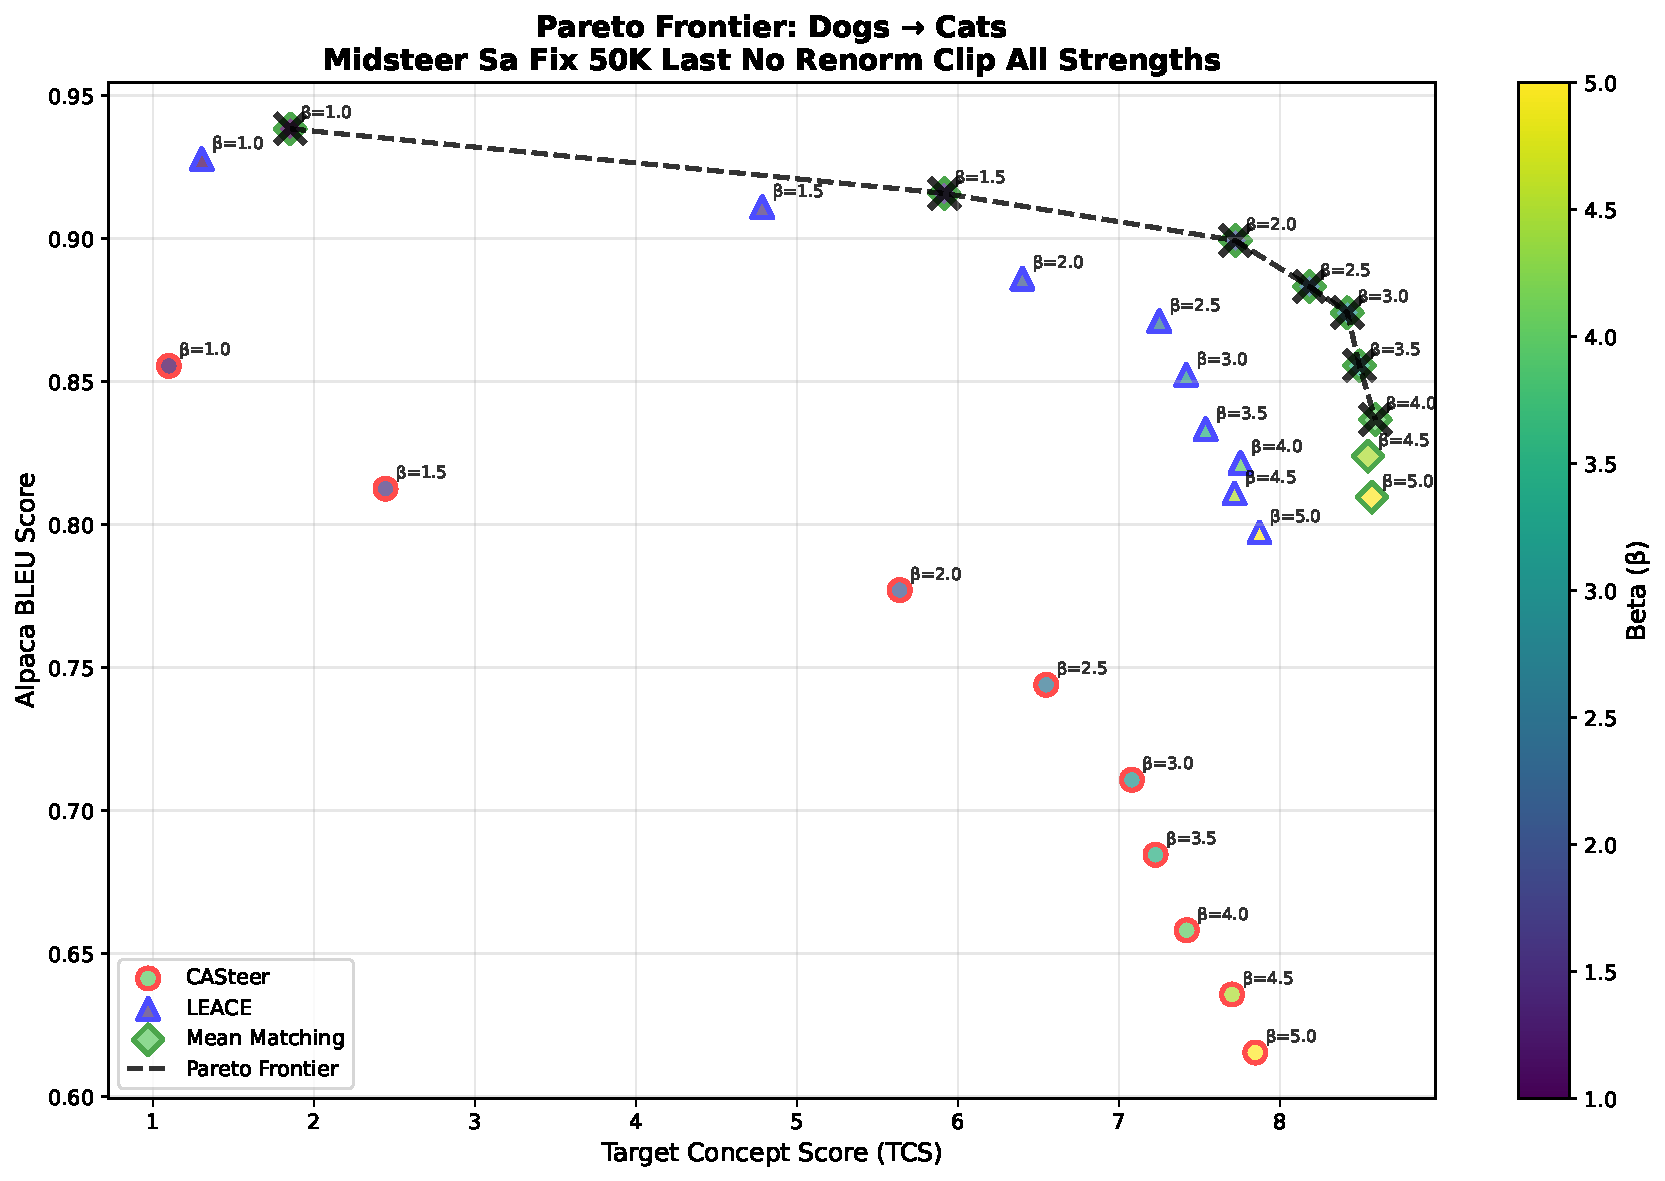
\includegraphics[width=0.9\linewidth,center]{pareto_plots/midsteer_sa_fix_50k_last_no_renorm_clip_all_strengths_dogs_to_cats_pareto_frontier.pdf}
    \caption{Pareto Efficiency Frontier for Dogs $\to$ Cats steering, with clipping}
    \label{fig:pareto_frontier_chart_dogs_cats_with_clipping}
\end{figure}

\begin{figure}[htbp]
    \centering
    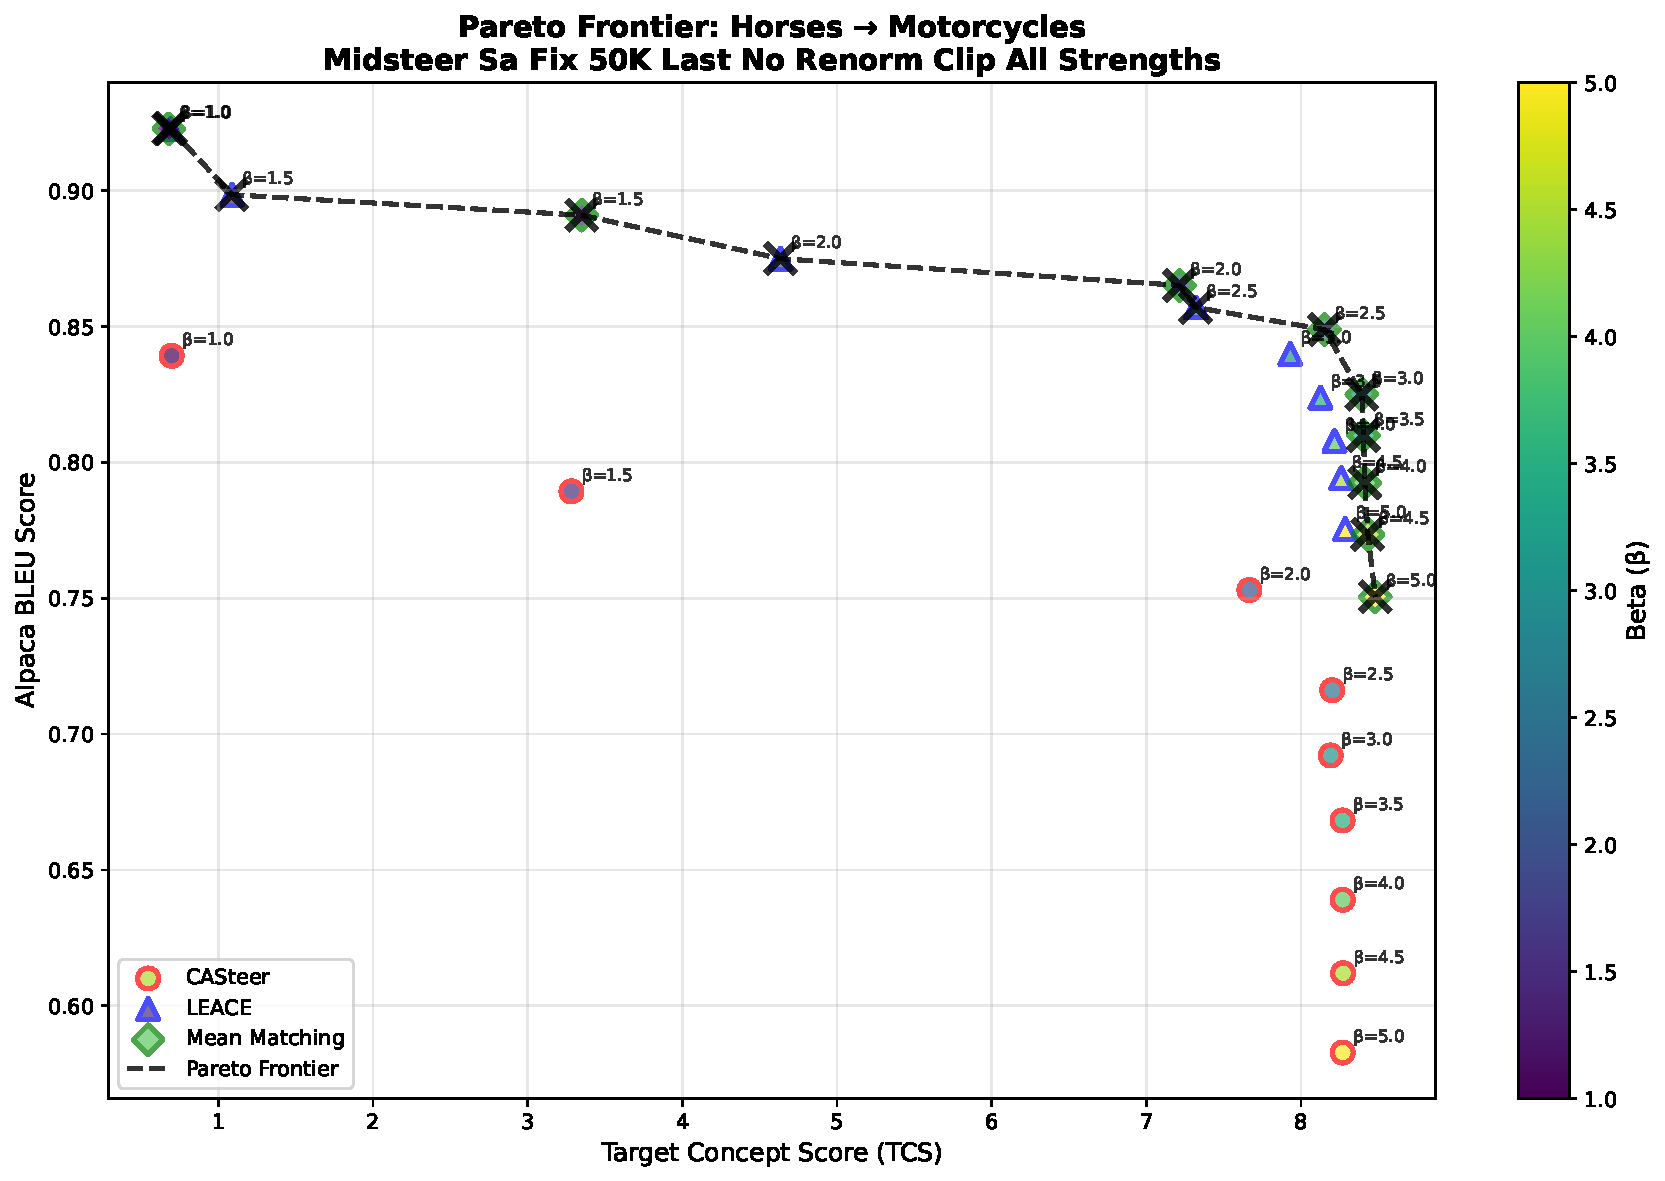
\includegraphics[width=0.9\linewidth,center]{pareto_plots/midsteer_sa_fix_50k_last_no_renorm_clip_all_strengths_horses_to_motorcycles_pareto_frontier.pdf}
    \caption{Pareto Efficiency Frontier for Horses $\to$ Motorcycles steering, with clipping}
    \label{fig:pareto_frontier_chart_horses_motorcycles_with_clipping}
\end{figure}

\begin{figure}[htbp]
    \centering
    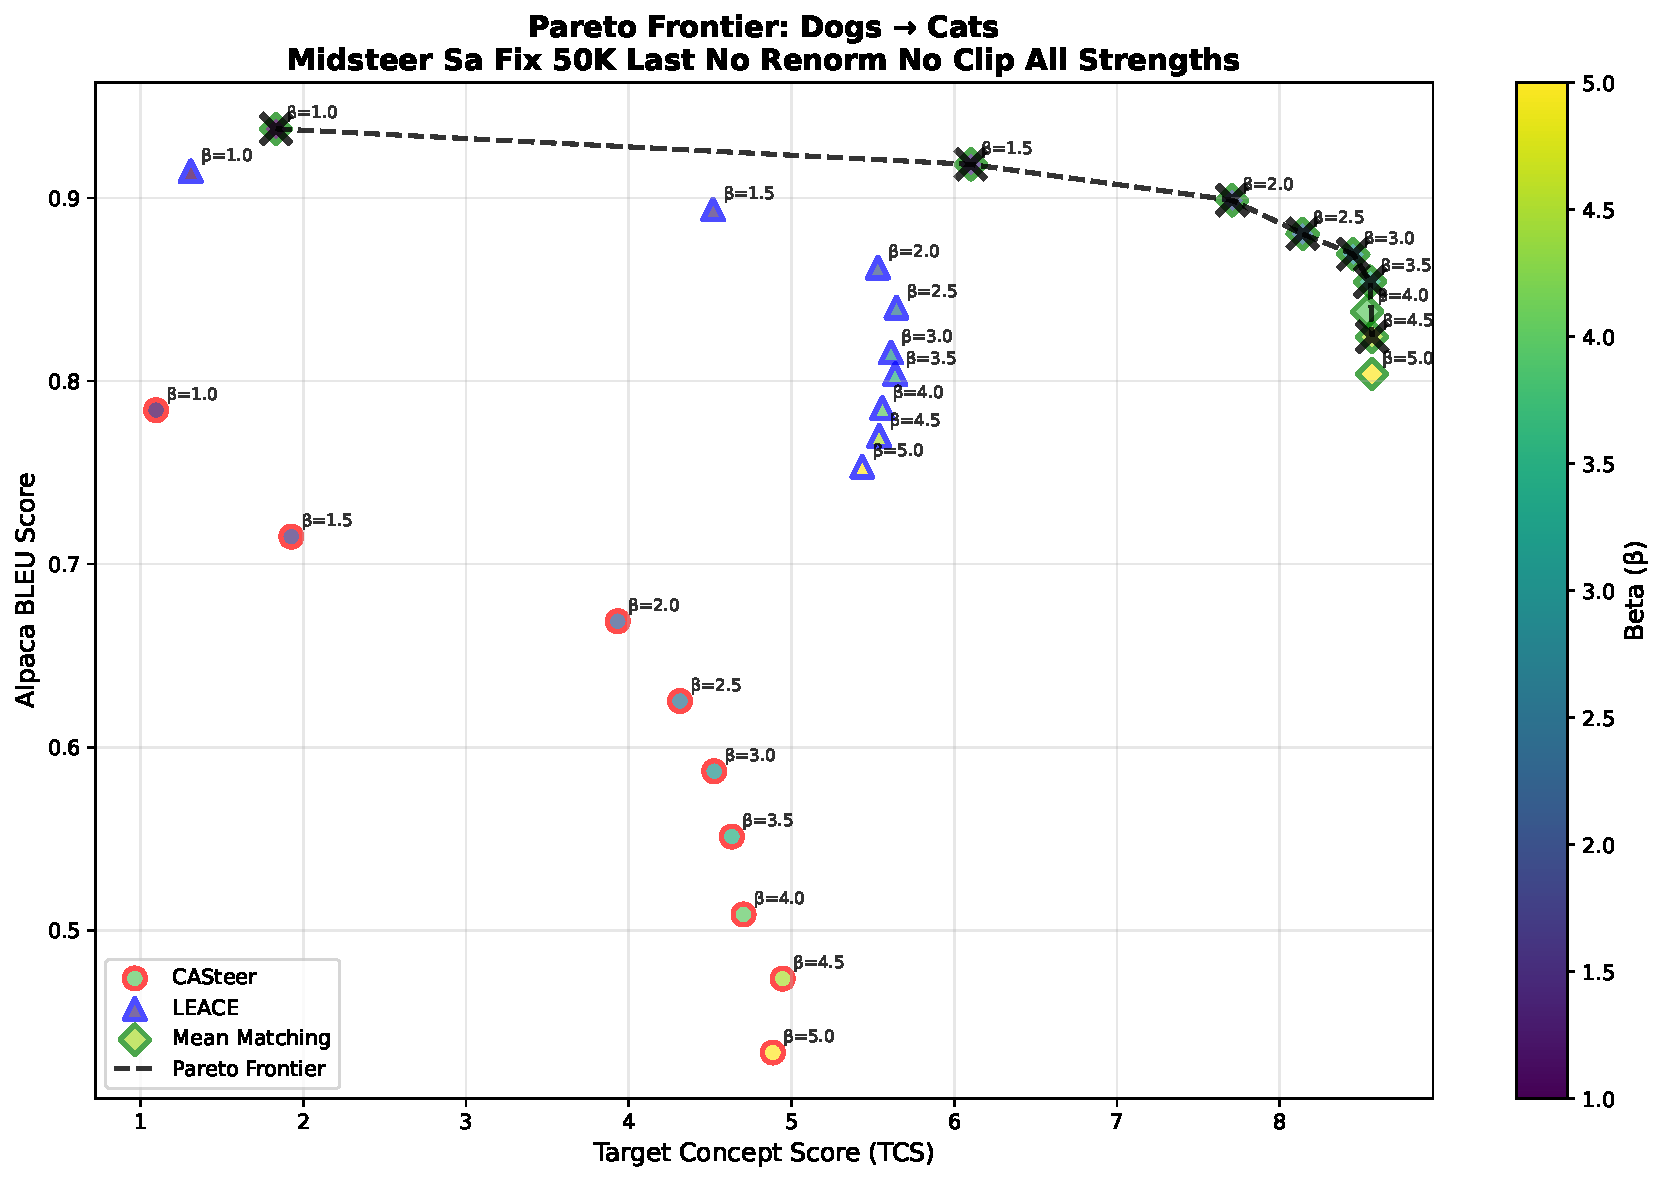
\includegraphics[width=0.9\linewidth,center]{pareto_plots/midsteer_sa_fix_50k_last_no_renorm_no_clip_all_strengths_dogs_to_cats_pareto_frontier.pdf}
    \caption{Pareto Efficiency Frontier for Dogs $\to$ Cats steering, without clipping}
    \label{fig:pareto_frontier_chart_dogs_cats_without_clipping}
\end{figure}

\begin{figure}[htbp]
    \centering
    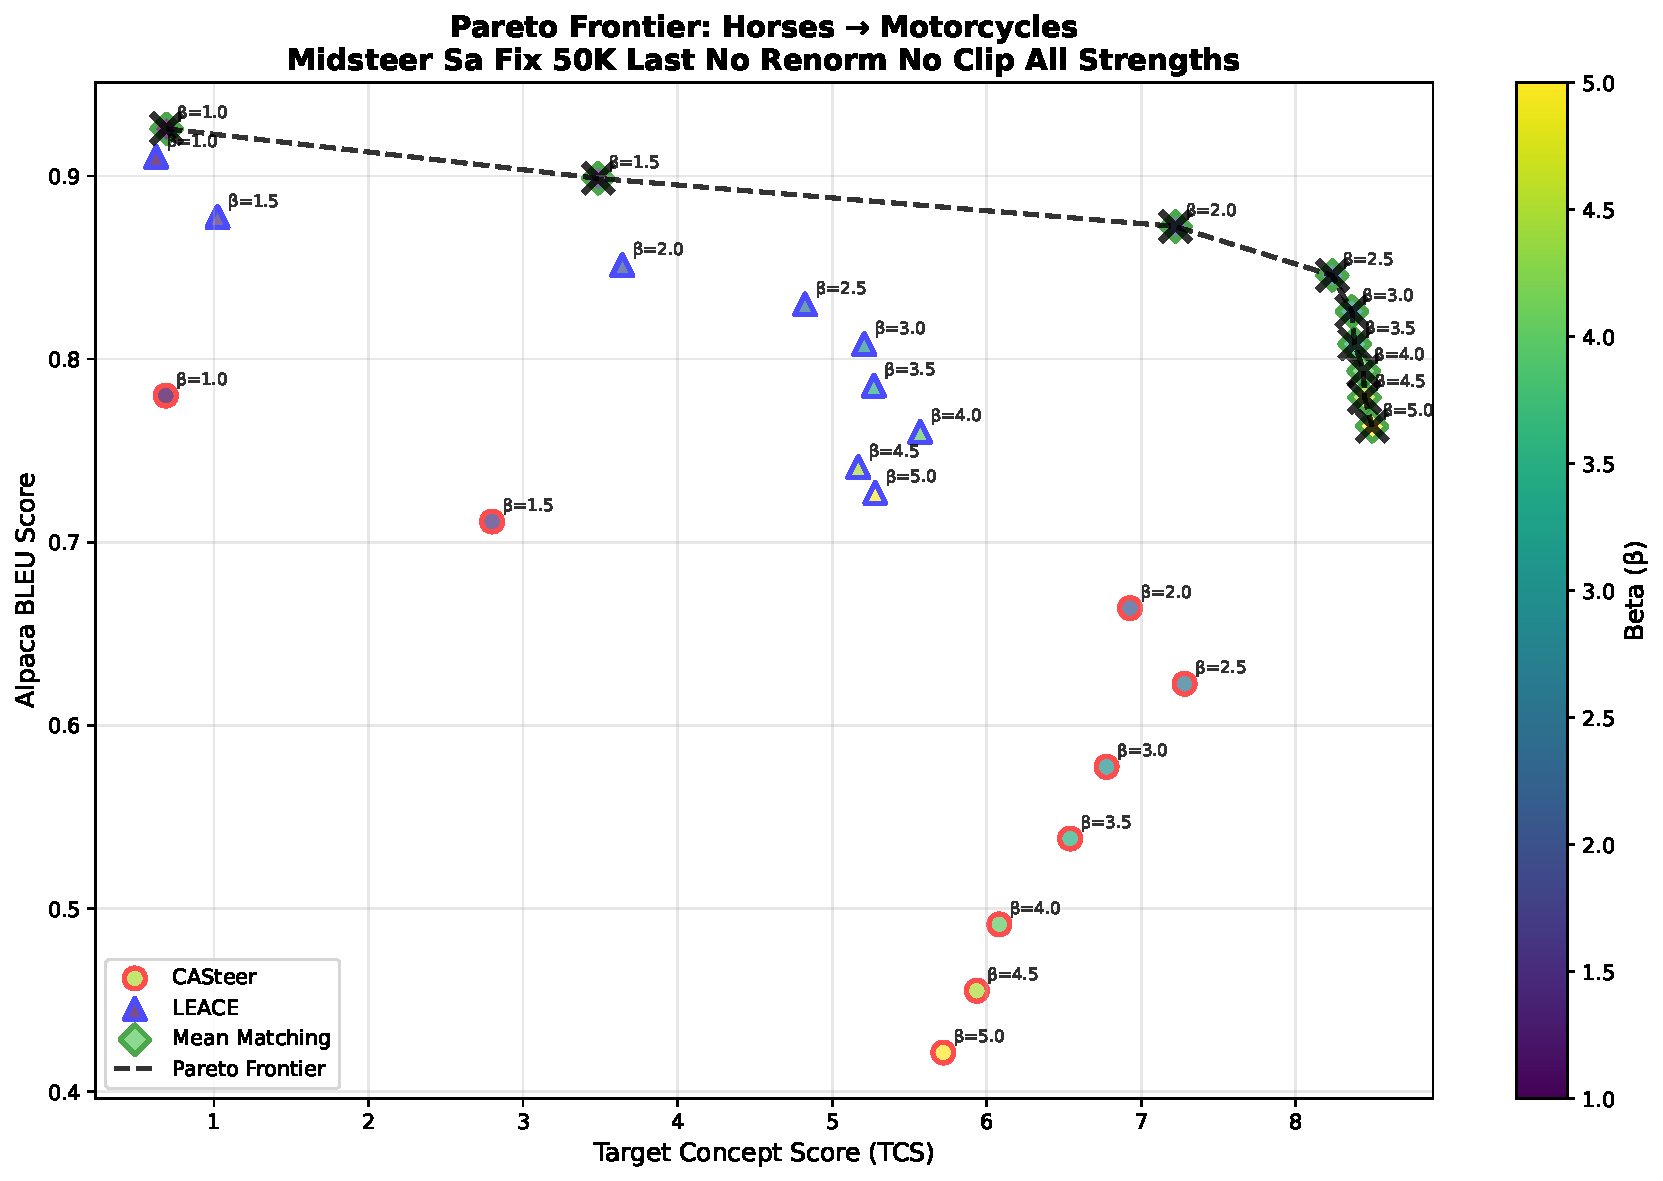
\includegraphics[width=0.9\linewidth,center]{pareto_plots/midsteer_sa_fix_50k_last_no_renorm_no_clip_all_strengths_horses_to_motorcycles_pareto_frontier.pdf}
    \caption{Pareto Efficiency Frontier for Horses $\to$ Motorcycles steering, without clipping}
    \label{fig:pareto_frontier_chart_horses_motorcycles_without_clipping}
\end{figure}

\begin{figure}[htbp]
    \centering
    
\includegraphics[width=1.3\linewidth,center]{pareto_plots/mixed_clip_comparison_dogs_to_cats_pareto_frontier.pdf}
    \caption{Pareto Efficiency Frontier for Dogs $\to$ Cats steering and mixed clipping use}
    \label{fig:pareto_frontier_chart_dogs_cats_mixed_clipping}
\end{figure}

\begin{figure}[htbp]
    \centering
    
\includegraphics[width=1.3\linewidth,center]{pareto_plots/mixed_clip_comparison_horses_to_motorcycles_pareto_frontier.pdf}
    \caption{Pareto Efficiency Frontier for Horse $\to$ Motorcycle steering and mixed clipping use}
    \label{fig:pareto_frontier_chart_horses_motorcycles_mixed_clipping}
\end{figure}

\subsubsection{Covariance comparison}

In this section, we try to find the optimal number of samples to estimate covariances. Since covariances are used for whitening, having more samples to estimate from might improve the ALPACA and MMLU results.

In figure \ref{covariance_comparison_midsteer-sa-fix-N-last-no-renorm-no-clip_combined-tasks_alpaca-bleu_beta-2.0} we can observe that the optimal number of covariances lies in 5 to 10 thousand, depending on the method.


\begin{figure}[htbp]
    \centering
    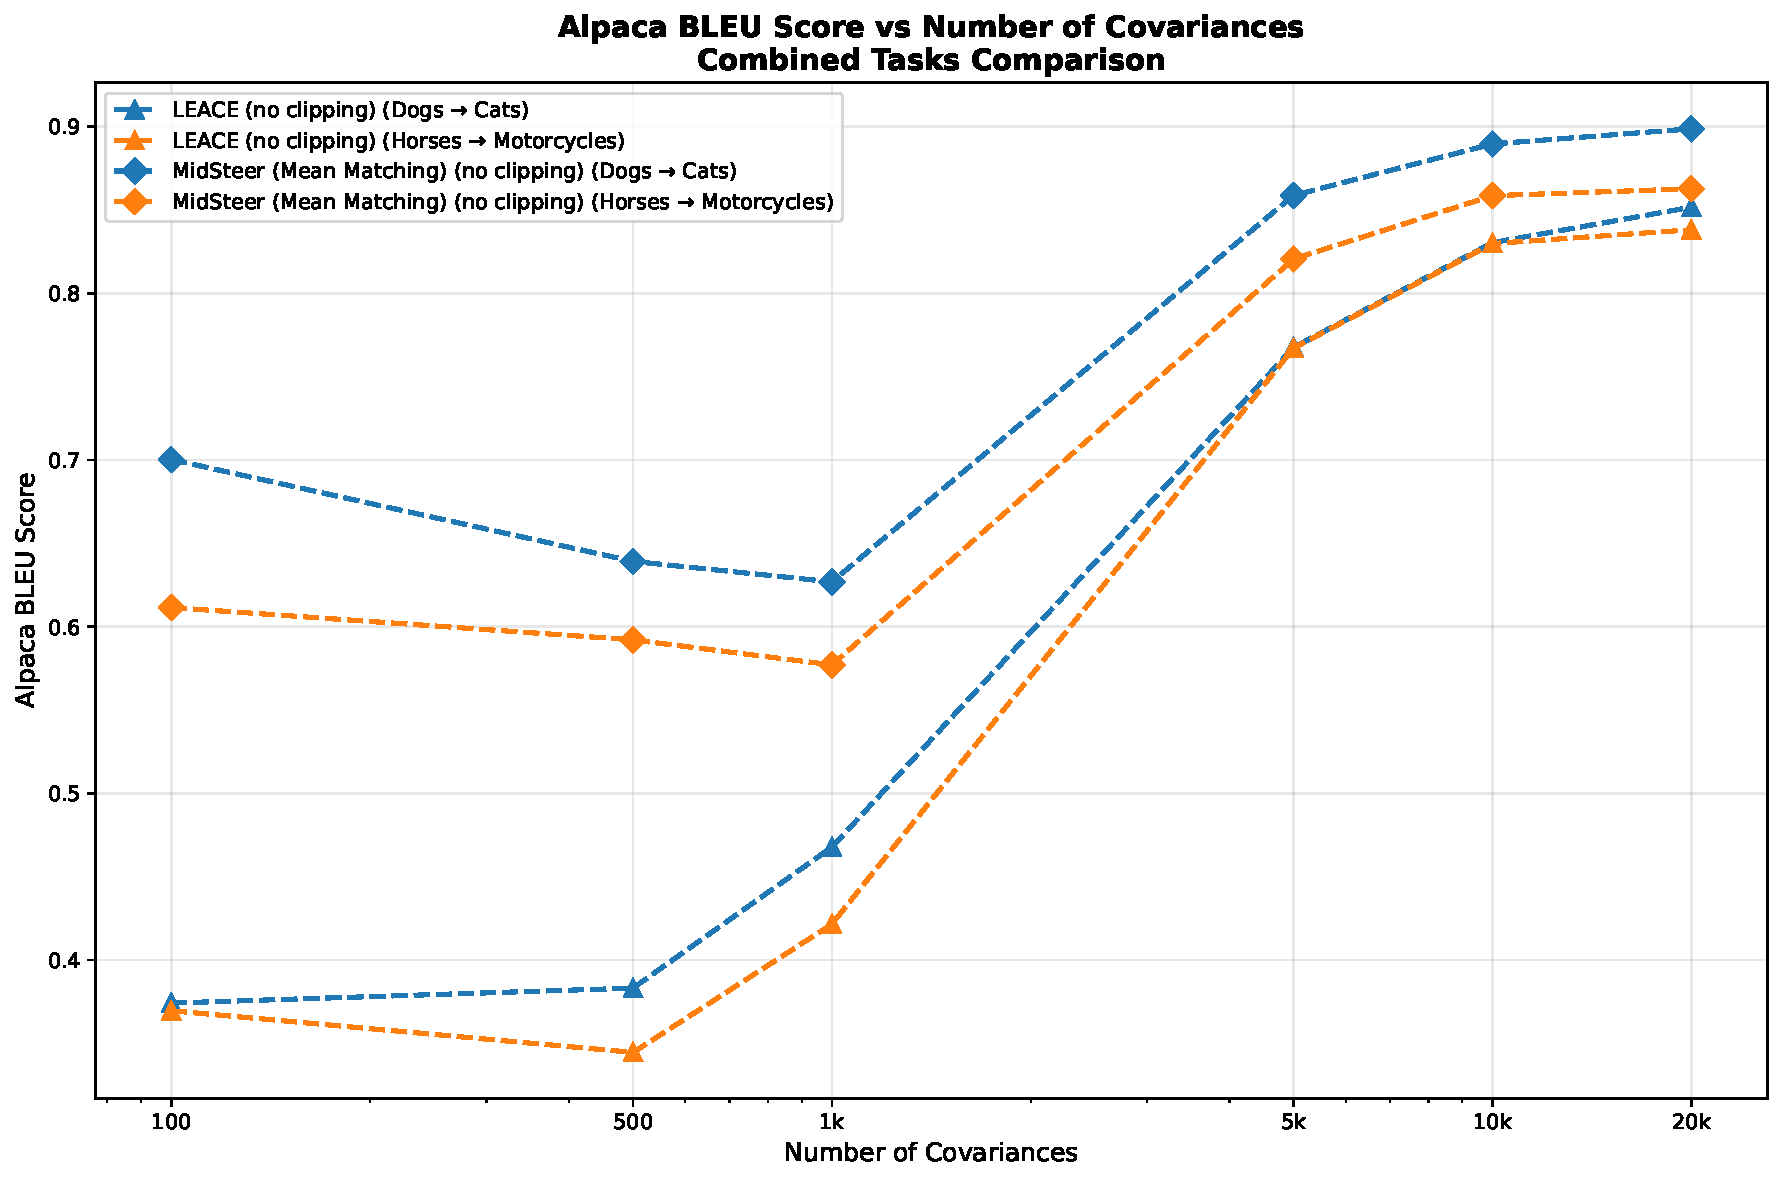
\includegraphics[width=1.1 \linewidth,center]{covariance_plots/covariance_comparison_midsteer-sa-fix-N-last-no-renorm-no-clip_combined-tasks_alpaca-bleu_beta-2.0.pdf}
    \caption{Alpaca BLEU scores on a held-out subset for different methods and different steering tasks. Covariances are estimated on a separate training subset using 100, 500, 1000, 5000, 10000, 20000 and 50000 samples.}
    \label{covariance_comparison_midsteer-sa-fix-N-last-no-renorm-no-clip_combined-tasks_alpaca-bleu_beta-2.0}
\end{figure}\n\n\begin{figure}[htbp]
    \centering
    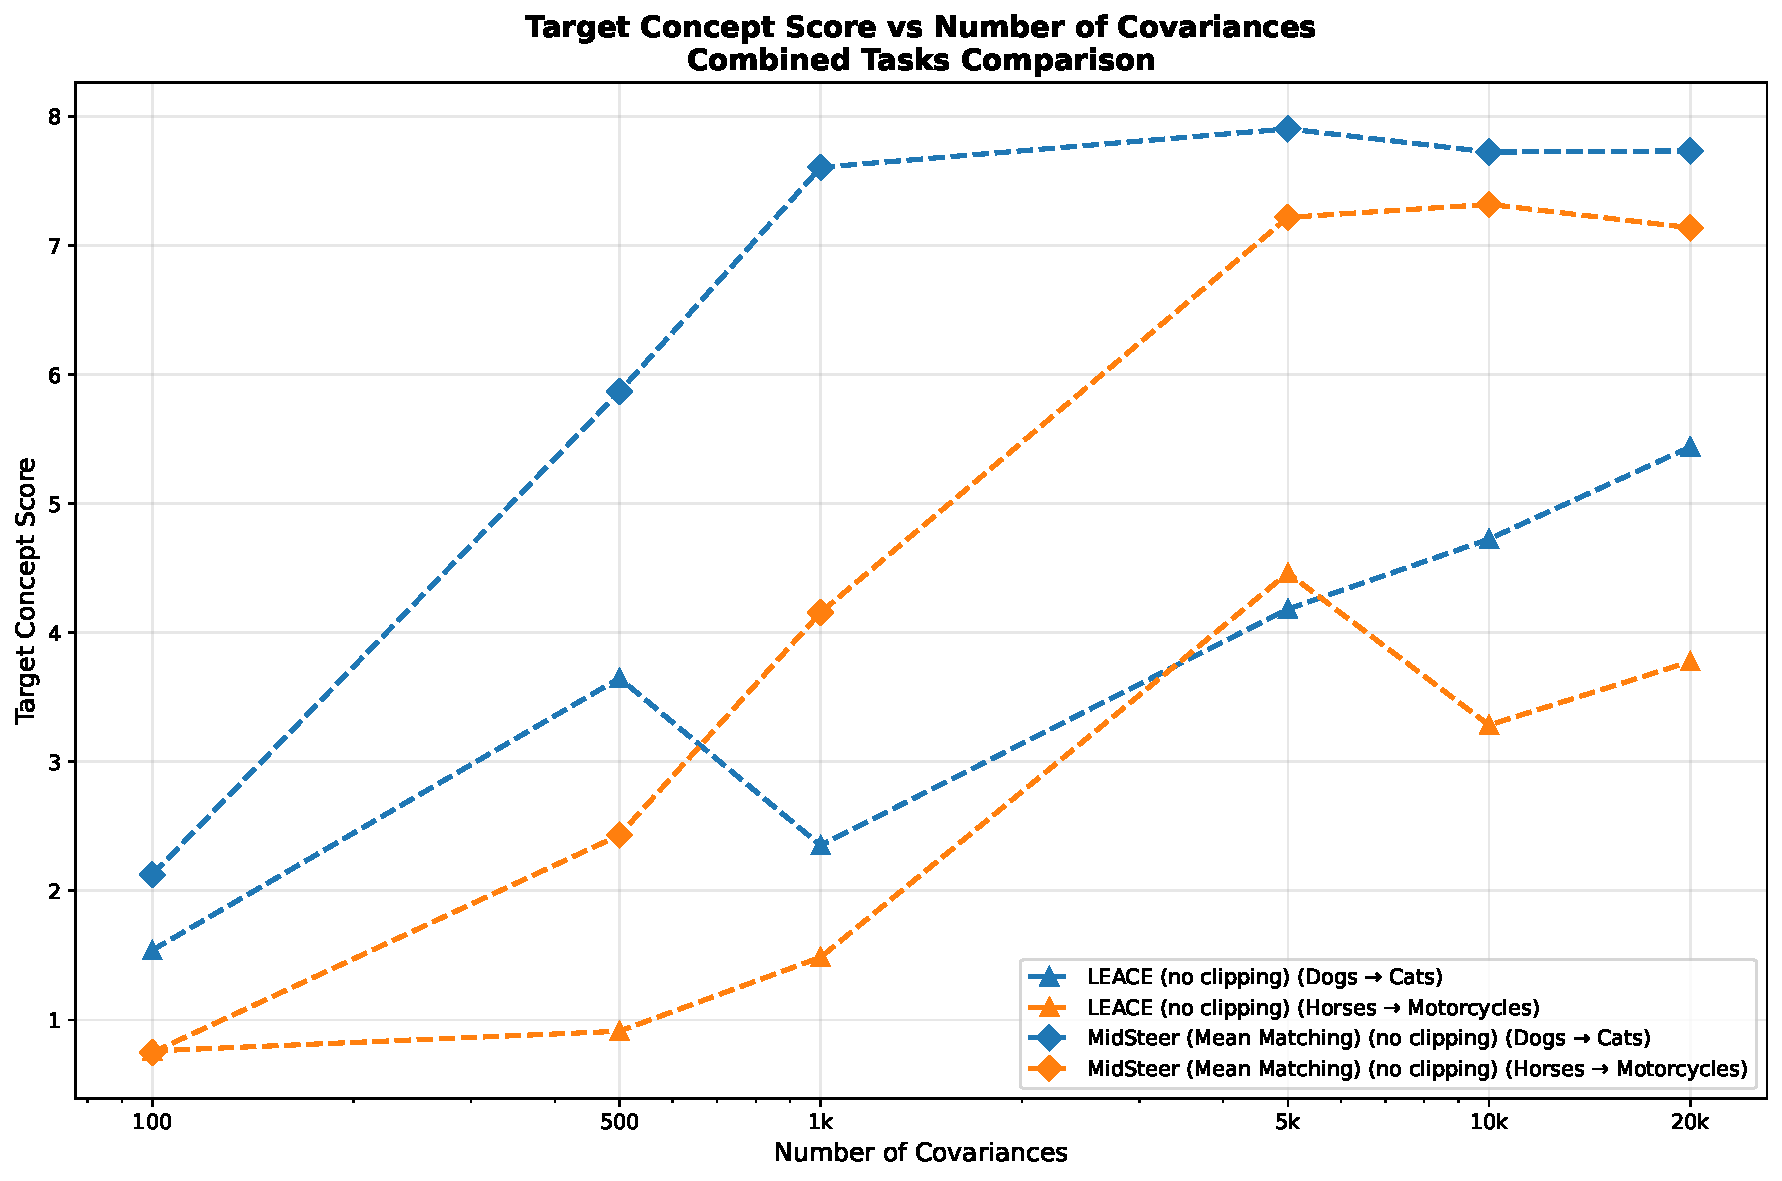
\includegraphics[width=1.1 \linewidth,center]{covariance_plots/covariance_comparison_midsteer-sa-fix-N-last-no-renorm-no-clip_combined-tasks_target-concept-score_beta-2.0.pdf}
    \caption{Alpaca BLEU scores on a held-out subset for different methods and different steering tasks. Covariances are estimated on a separate training subset using 100, 500, 1000, 5000, 10000, 20000 and 50000 samples.}
    \label{covariance_comparison_midsteer-sa-fix-N-last-no-renorm-no-clip_combined-tasks_target-concept-score_beta-2.0}
\end{figure}

\subsubsection{Implicit concepts}

In this section, we compare how methods work on an implicitly defined concept. For horse, we used implicit definitions as "knight's riding mammal", "large equine". For dog we used "man's best friend" and "domesticated canine". The results are presented in tables \ref{tab:implicitconcept_knight_s_riding_mammal_horsestomotorcycles_avg2} and \ref{tab:implicitconcept_man_s_best_friend_dogstocats_avg2}. All methods loose some peformance when switching to implicitly deifned concept, but MidSteer maintains its advantage over other methods.



\begin{table}[htbp]
\centering
\caption{Comprehensive Results: Implicit Concept (avg. of 2 concepts) - Horses$\to$Motorcycles}
\label{tab:implicitconcept_knight_s_riding_mammal_horsestomotorcycles_avg2}
\begin{tabular}{l|l|cccccc|}
\hline
Method & $\beta$ & \multicolumn{6}{c|}{SCS (avg. 2 implicit concepts)} \\
 &  & SCS & TCS & A-BLEU & A-BertF1 & M-BLEU & M-BertF1 \\
\hline
CASteer\textsuperscript{†} & 2.0 & 7.01 & 4.69 & 0.753 & 0.974 & 0.647 & 0.954 \\
 & 3.0 & 6.09 & 5.40 & 0.692 & 0.968 & 0.564 & 0.944 \\
 & 4.0 & 5.34 & 5.79 & 0.639 & 0.961 & 0.507 & 0.937 \\
\hline
LEACE\textsuperscript{†} & 2.0 & \textbf{7.50} & 4.32 & \textbf{0.875} & \textbf{0.987} & \textbf{0.806} & \textbf{0.975} \\
 & 3.0 & 6.68 & 5.02 & 0.840 & 0.984 & \underline{0.744} & \underline{0.967} \\
 & 4.0 & 5.77 & 5.31 & 0.808 & 0.980 & 0.696 & 0.961 \\
\hline
Mean Matching\textsuperscript{‡} & 2.0 & \underline{7.05} & 4.92 & \underline{0.865} & \underline{0.986} & 0.701 & 0.961 \\
 & 3.0 & 5.81 & \underline{5.85} & 0.825 & 0.982 & 0.610 & 0.949 \\
 & 4.0 & 5.24 & \textbf{6.43} & 0.793 & 0.978 & 0.545 & 0.941 \\
\hline
\end{tabular}
\\[0.5em]
\footnotesize
\textsuperscript{†} With clipping \quad \textsuperscript{‡} Without clipping (fully compliant matrix form)
\end{table}

\begin{table}[htbp]
\centering
\caption{Comprehensive Results: Implicit Concept (avg. of 2 concepts) - Dogs$\to$Cats}
\label{tab:implicitconcept_man_s_best_friend_dogstocats_avg2}
\begin{tabular}{l|l|cccccc|}
\hline
Method & $\beta$ & \multicolumn{6}{c|}{SCS (avg. 2 implicit concepts)} \\
 &  & SCS & TCS & A-BLEU & A-BertF1 & M-BLEU & M-BertF1 \\
\hline
CASteer\textsuperscript{†} & 2.0 & \textbf{6.20} & 4.86 & 0.777 & 0.976 & 0.752 & 0.968 \\
 & 3.0 & 5.38 & 6.62 & 0.711 & 0.969 & 0.684 & 0.959 \\
 & 4.0 & 5.17 & 7.16 & 0.658 & 0.963 & 0.616 & 0.950 \\
\hline
LEACE\textsuperscript{†} & 2.0 & \underline{5.47} & 6.31 & \underline{0.886} & \underline{0.988} & \textbf{0.882} & \textbf{0.985} \\
 & 3.0 & 5.15 & 7.35 & 0.852 & 0.985 & \underline{0.837} & \underline{0.979} \\
 & 4.0 & 4.90 & 7.82 & 0.822 & 0.982 & 0.802 & 0.974 \\
\hline
Mean Matching\textsuperscript{‡} & 2.0 & 4.94 & 7.65 & \textbf{0.899} & \textbf{0.990} & 0.789 & 0.972 \\
 & 3.0 & 4.36 & \underline{8.26} & 0.874 & 0.987 & 0.727 & 0.964 \\
 & 4.0 & 4.19 & \textbf{8.46} & 0.837 & 0.983 & 0.669 & 0.957 \\
\hline
\end{tabular}
\\[0.5em]
\footnotesize
\textsuperscript{†} With clipping \quad \textsuperscript{‡} Without clipping (fully compliant matrix form)
\end{table}